% Provenance (never printed): old premiere S material on subduction (Wadati-Benioff
% planes, density of the old lithosphere, slab pull, transformation of the slab at
% depth: blueschist and eclogite; anatomy of an active margin). Sections from
% figdata/grade-11/slab_sections.py (USGS ComCat M >= 6 1976-2025, PB2002 steps,
% Seton 2020 ages); plate speeds from plate_velocities.py (NNR-MORVEL56 RMS).
% Metamorphism is defined in g12.03, the volcanic arc in g12.04: named only here.
\chapter{Subductiezones}\label{ch:g11:subduction-zones}

Onder de eilanden van Tonga, in het zuidwesten van de Grote Oceaan, beeft de Aarde
veel dieper dan waar ook. Van de zevenduizend aardbevingen met magnitude
6 of meer die tussen 1976 en 2025 wereldwijd zijn geregistreerd, vond de diepste
\qty{688}{km} diep plaats, en de doorsnede door Tonga in dit hoofdstuk bevat schokken tot
ongeveer \qty{671}{km}. Op zulke diepten is het gesteente heet en staat het onder enorme
druk; het zou langzaam moeten vloeien, zoals de \omterm{def:g11:lithosphere-asthenosphere:lithosphere}{asthenosfeer}, en niet breken. Toch
breekt het. Dit hoofdstuk legt uit wat daar breekt: een plaat koude oceaanbodem
die terug in de mantel zakt.
% ledger: data:usgs-comcat (catalogue_maxdepth 688; tonga_maxdepth 670.8, slab_sections.py)

\begin{recall}
Bij een convergente grens bewegen twee platen naar elkaar toe; langs sommige
ervan liggen diepe troggen (Boek 1, jaar 7 en 8). De magnitude van een aardbeving
meet haar grootte, en een aardbeving onder de zee kan een tsunami veroorzaken
(Boek 1, jaar 7). De snelheid van een plaat ten opzichte van een andere is het
verschil van hun snelheden (\cref{ch:g11:plate-motions}). Oceaanbodem
zakt weg naarmate hij ouder wordt, en na zo'n 60 miljoen jaar is zijn \omterm{def:g11:lithosphere-asthenosphere:lithosphere}{lithosfeer}, ongeveer
\qty{100}{km} dik, dichter dan de \omterm{def:g11:lithosphere-asthenosphere:lithosphere}{asthenosfeer} eronder
(\cref{ch:g11:ocean-ridges}). Seismische golven tonen een scherpe verandering in de
mantel op ongeveer \qty{670}{km} (\cref{ch:g11:seismic-structure}). Een metamorf
gesteente is een gesteente dat in vaste toestand is omgevormd (Boek 1, jaar 6).
\end{recall}
% ledger: data:prem (670 km), ps77:depth-age

\section{Troggen en hellende aardbevingszones}

De meeste aardbevingen zijn ondiep: in de catalogus van magnitude 6 of meer sinds
1976 is maar ongeveer één op vijf dieper dan \qty{70}{km}, en één op vijftien
dieper dan \qty{300}{km}. De kaart hieronder laat zien waar de diepe liggen.
% values (slab_sections.py): frac_deeper_70 0.21, frac_deeper_300 0.069; data:usgs-comcat

\begin{omfigure}
\begin{tikzpicture}
\begin{axis}[ommap, width=\linewidth, xtick={-180,-90,...,180}, ytick={-60,0,60},
  legend style={font=\scriptsize, at={(0.5,-0.13)}, anchor=north, legend columns=3,
    /tikz/every even column/.append style={column sep=6pt}}]
\addplot[fill=omLithAlluv, draw=black!45, line width=0.2pt, forget plot] table {figdata/out/shared-geo-land.dat};
\addplot[black!70, line width=0.5pt, forget plot] table {figdata/out/shared-geo-school-subduction.dat};
\addplot[fill=black!70, draw=none, forget plot] table {figdata/out/shared-geo-school-teeth.dat};
% computed in figdata/grade-11/slab_sections.py; ledger: data:usgs-comcat, data:pb2002
\addplot[only marks, mark=*, mark size=0.55pt, black!45] table[x=lon, y=lat] {figdata/out/grade-11-slab_sections-world-shallow.dat};
\addplot[only marks, mark=*, mark size=0.8pt, omProp] table[x=lon, y=lat] {figdata/out/grade-11-slab_sections-world-mid.dat};
\addplot[only marks, mark=*, mark size=1.1pt, omThm] table[x=lon, y=lat] {figdata/out/grade-11-slab_sections-world-deep.dat};
\legend{{ondieper dan \qty{70}{km}}, {70 tot \qty{300}{km}}, {dieper dan \qty{300}{km}}}
\end{axis}
\end{tikzpicture}

{\small Aardbevingen met magnitude 6.5 of meer, 1976--2025 (2192 schokken),
gekleurd naar diepte, met de troggen (zwarte lijn, driehoekjes op de plaat die
eroverheen schuift). Middeldiepe en diepe aardbevingen liggen alleen langs sommige
troggen, altijd aan de kant van de bovenliggende plaat. Gegevens: aardbevingscatalogus
van de USGS; plaatgrenzen van Bird (2003); land van Natural Earth.}
\end{omfigure}
% values: world_n_m65 2192, world_deep_n 197 (slab_sections.py)

De diepe aardbevingen liggen niet verspreid: ze volgen de troggen van het
westen van de Grote Oceaan, van Kamtsjatka tot Japan, de Marianen, Indonesië en Tonga,
en de trog langs de westkust van Zuid-Amerika; en ze liggen altijd aan
één kant van de trog, onder de plaat die niet wegzakt.

\begin{definition}[Subductie; subductiezone]\label{def:g11:subduction-zones:subduction}
\emph{Subductie}\index{subductie} is het wegzakken van een plaat \omterm{def:g11:ocean-ridges:oceanic-lithosphere}{oceanische
lithosfeer} onder een andere plaat, terug in de mantel. Een
\emph{subductiezone}\index{subductiezone} is een convergente plaatgrens waar subductie
plaatsvindt; ze is aan het oppervlak gemarkeerd door een trog.
\end{definition}

\begin{definition}[Wadati--Benioffzone]\label{def:g11:subduction-zones:benioff}
Een \emph{Wadati--Benioffzone}\index{Wadati--Benioffzone} is de hellende
band van aardbevingen die bij een trog begint en steeds dieper gaat onder
de bovenliggende plaat, tot wel ongeveer \qty{700}{km}.
\end{definition}
% ledger: frohlich87:wadati

\begin{history}[Wadati en Benioff]
In de jaren 1920 betoogden vooraanstaande seismologen dat aardbevingen alleen
in de eerste paar tientallen kilometers konden plaatsvinden: de diepere Aarde, zo
redeneerden ze, had geen sterkte om de spanning op te slaan. De Japanse seismoloog Kiyoo Wadati, die werkte met het
dichte netwerk van stations van de Japanse meteorologische dienst, leverde vanaf 1928
het eerste overtuigende bewijs dat sommige aardbevingen honderden
kilometers diep liggen: een van de schokken die hij bestudeerde, in januari 1927, lag
\qty{420}{km} diep. In 1935 publiceerde hij de eerste kaart van de diepten van
deze aardbevingen, getekend als hoogtelijnen, en merkte hij op dat de steeds dieper
wordende zone evenwijdig liep aan de rij actieve vulkanen. In 1949 en 1954 liet de
Amerikaanse seismoloog Hugo Benioff zien dat de aardbevingen onder de Andes en de
Tonga--Kermadeceilanden langs zones liggen die diepten van
ongeveer \qty{700}{km} bereiken. De zones heetten eerst Benioffzones, in 1967; de
naam \omterm{def:g11:subduction-zones:benioff}{Wadati--Benioffzone}, die beide hun verdiende eer geeft, volgt een voorstel
van de Japanse geofysicus Seiya Uyeda uit 1971.
\end{history}
% ledger: frohlich87:wadati

\begin{method}[Een aardbevingsdoorsnede lezen]\label{met:g11:subduction-zones:section}
\begin{enumerate}
  \item Kies een lijn loodrecht op de trog, van de trog naar de
        bovenliggende plaat, en houd de aardbevingen binnen een band aan weerszijden
        ervan.
  \item Zet elke aardbeving uit op haar afstand langs de lijn (horizontaal)
        en op haar diepte (verticaal, naar beneden).
  \item Zoek de hellende band; trek de rechte lijn die hem het best
        volgt.
  \item Lees de helling van de band af uit twee punten van de lijn (propositie
        hieronder).
\end{enumerate}
\end{method}

\begin{omfigure}
\begin{tikzpicture}
\begin{axis}[omrecord, omdepth, name=tonga, width=0.5\linewidth, height=6.4cm,
  xmin=-150, xmax=900, ymin=0, ymax=720, xlabel={afstand tot de trog (\unit{km})},
  ylabel={diepte (\unit{km})}, title={\small Tonga}, clip=false]
% computed in figdata/grade-11/slab_sections.py; ledger: data:usgs-comcat, data:pb2002
\addplot[only marks, mark=*, mark size=1.2pt, black!65] table[x=x, y=depth] {figdata/out/grade-11-slab_sections-tonga.dat};
\addplot[omProp, line width=1pt, domain=135.7:761.6, samples=2] {-23.568 + 0.91068*x};
\addplot[only marks, mark=triangle*, mark size=3pt, omDef] coordinates {(0,0)};
\node[font=\scriptsize, anchor=south west, text=omDef] at (axis cs:10,8) {trog};
\node[font=\scriptsize, anchor=west, text=omProp, align=left] at (axis cs:300,560) {helling\\\ang{42}};
\end{axis}
\begin{axis}[omrecord, omdepth, at={(tonga.east)}, anchor=west, xshift=0.3cm, width=0.5\linewidth, height=6.4cm,
  xmin=-150, xmax=900, ymin=0, ymax=720, xlabel={afstand tot de trog (\unit{km})},
  yticklabels={}, title={\small Andes, bij \ang{21} ZB}, clip=false]
\addplot[only marks, mark=*, mark size=1.2pt, black!65] table[x=x, y=depth] {figdata/out/grade-11-slab_sections-andes.dat};
\addplot[omProp, line width=1pt, domain=253.0:900, samples=2] {-88.745 + 0.74613*x};
\addplot[only marks, mark=triangle*, mark size=3pt, omDef] coordinates {(0,0)};
\node[font=\scriptsize, anchor=south west, text=omDef] at (axis cs:10,8) {trog};
\node[font=\scriptsize, anchor=west, text=omProp, align=left] at (axis cs:300,560) {helling\\\ang{37}};
\end{axis}
\end{tikzpicture}

{\small Aardbevingsdoorsneden loodrecht op twee troggen: aardbevingen met
magnitude 6 of meer, 1976--2025, binnen \qty{150}{km} van de doorsnedelijn,
uitgezet op hun afstand tot de trog (naar de bovenliggende plaat) en
hun diepte. Oranje: de rechte lijn die de aardbevingen tussen 100 en
\qty{600}{km} diepte het best volgt. Onder Tonga reikt de band tot onder
\qty{670}{km}. Gegevens: aardbevingscatalogus van de USGS; posities van de troggen van Bird (2003).}
\end{omfigure}
% values (slab_sections.py): tonga_dip 42.3, fit -23.568 + 0.91068 x (77 events);
% andes_dip 36.7, fit -88.745 + 0.74613 x; trench points tonga (-173.31, -20.395),
% andes (-71.286, -21.01)

\begin{proposition}[De helling van een slab uit een aardbevingsdoorsnede]\label{prop:g11:subduction-zones:dip}
Als twee punten van de lijn die een \omterm{def:g11:subduction-zones:benioff}{Wadati--Benioffzone} volgt, op
horizontale afstanden $x_1 < x_2$ van de trog en op diepten $z_1$ en $z_2$ liggen,
voldoet haar helling $\delta$, de hoek die ze met de horizontaal maakt, aan
\[
  \tan \delta = \frac{z_2 - z_1}{x_2 - x_1}.
\]
\end{proposition}

\begin{proof}
De twee punten en het punt op diepte $z_1$ verticaal boven het tweede
vormen een rechthoekige driehoek. Zijn horizontale zijde is $x_2 - x_1$, zijn verticale zijde
$z_2 - z_1$, en de hoek bij het eerste punt is de helling. De tangens van een
hoek van een rechthoekige driehoek is de overstaande zijde gedeeld door de aanliggende zijde.
\end{proof}

\begin{example}[De helling onder Tonga]\label{ex:g11:subduction-zones:dip}
De lijn van de doorsnede door Tonga ligt \qty{250}{km} diep op \qty{300}{km} van
de trog en \qty{614}{km} diep op \qty{700}{km}. Dus
$\tan\delta = (614 - 250)/(700 - 300) = 364/400 = 0.91$, en
$\delta \approx \ang{42}$. Onder de Andes, op \ang{21}~ZB, geeft dezelfde
methode ongeveer \ang{37}.
\end{example}
% values: tonga line at 300 km 249.6, at 700 km 613.9 (slab_sections.py)

De \omterm{def:g11:subduction-zones:benioff}{Wadati--Benioffzone} tekent een plaat die naar beneden gaat. Ondiepe aardbevingen
vinden plaats waar de twee platen langs elkaar schuiven, dicht bij de trog; diepere
vinden plaats in de wegzakkende plaat zelf.

\section{Waarom oude lithosfeer wegzakt}

\begin{definition}[Slab]\label{def:g11:subduction-zones:slab}
Een \emph{slab}\index{slab} is het deel van een plaat dat bij een \omterm{def:g11:subduction-zones:subduction}{subductiezone} al in
de mantel is gezakt: een plaat \omterm{def:g11:ocean-ridges:oceanic-lithosphere}{oceanische lithosfeer} van ongeveer
honderd kilometer dik, die schuin onder de bovenliggende plaat ligt.
\end{definition}

Wat naar beneden gaat, is oude oceaanbodem. Volgens de ouderdom van de oceaanbodem
is de bodem die de Japantrog bereikt, ten oosten van Japan, ongeveer 133 miljoen jaar oud,
de bodem die de Tongatrog bereikt ongeveer 99 miljoen jaar; zelfs de
bodem die de Andes bereikt, een van de jongste die wegzakken, is ongeveer 49
miljoen jaar oud. Zulke oude \omterm{def:g11:lithosphere-asthenosphere:lithosphere}{lithosfeer} is koud en dik, en, afgezien van
zijn lichte korst, dichter dan de \omterm{def:g11:lithosphere-asthenosphere:lithosphere}{asthenosfeer}: zodra één rand ervan
naar beneden begint te gaan, trekt zijn eigen gewicht hem erin.
% values (slab_sections.py): japan_age 133.1, tonga_age 98.8, andes_age 48.8 (median of the
% 1-degree cells 100-400 km seaward of the trench point); ledger data:b2-seafloor-age

\begin{definition}[Slabtrek; rugduw]\label{def:g11:subduction-zones:slab-pull}
\emph{Slabtrek}\index{slabtrek} is de kracht die een wegzakkende \omterm{def:g11:subduction-zones:slab}{slab}, dichter
dan de mantel eromheen, uitoefent op de rest van zijn plaat, en die haar naar
de trog trekt. \emph{Rugduw}\index{rugduw} is de kracht die een
plaat van een rug wegduwt, waar de jonge, hete \omterm{def:g11:lithosphere-asthenosphere:lithosphere}{lithosfeer} hoog op zijn
opgeheven rug staat en langs de helling naar beneden glijdt.
\end{definition}

Welke van de twee is belangrijker? In 1975 berekenden Donald Forsyth en Seiya Uyeda
de sterkte van elke kracht uit de snelheden en de vormen van
de platen: de krachten op de wegzakkende \omterm{def:g11:subduction-zones:slab}{slabs} bepalen de snelheid van de oceanische platen,
en zijn ongeveer tien keer sterker dan elke andere kracht. De
plaatsnelheden van vandaag laten het duidelijk zien.
% ledger: fu75:slab-pull

\begin{omfigure}
\begin{tikzpicture}
\begin{axis}[omrecord, ybar, bar width=9pt, width=0.86\linewidth, height=5.6cm,
  ymin=0, ymax=85, xmin=-0.7, xmax=12.7, bar shift=0pt, ylabel={gemiddelde snelheid (\unit{mm} per jaar)},
  xtick={0,...,12}, xticklabel style={rotate=50, anchor=east, font=\scriptsize},
  xticklabels={Cocos, Nazca, Pacifisch, Australië, Filipijnse Zee, Arabië, Somalië,
    Nubië, Eurazië, Noord-Amerika, Antarctica, Caribisch, Zuid-Amerika},
  ymajorgrids, xmajorgrids=false]
% computed in figdata/grade-11/slab_sections.py from plate_velocities.POLES (nnr56:rms)
\addplot[fill=omProp, draw=omProp!70!black] table[x=idx, y expr=\thisrow{slab}*\thisrow{rms}] {figdata/out/grade-11-slab_sections-speeds.dat};
\addplot[fill=omDef!35, draw=omDef] table[x=idx, y expr=(1-\thisrow{slab})*\thisrow{rms}] {figdata/out/grade-11-slab_sections-speeds.dat};
\node[font=\scriptsize, text=omProp!80!black, anchor=south] at (axis cs:2,76) {aan de plaat hangt een slab};
\node[font=\scriptsize, text=omDef, anchor=south] at (axis cs:9,50) {geen lange slab};
\end{axis}
\end{tikzpicture}

{\small De gemiddelde snelheid van dertien grote platen (kwadratisch gemiddelde over
de plaat, in een stelsel waarin de \omterm{def:g11:lithosphere-asthenosphere:lithosphere}{lithosfeer} als geheel niet draait).
Oranje: platen waaraan langs een lang stuk rand een wegzakkende \omterm{def:g11:subduction-zones:slab}{slab} hangt;
blauw: platen zonder. India is weggelaten: zijn noordrand is een
botsingszone. Gegevens: NNR-MORVEL56 (Argus, Gordon en DeMets,
2011).}
\end{omfigure}
% ledger: nnr56:rms; the bars of a class are drawn at 0 for the other (two series on one axis)

\begin{proposition}[Platen die aan slabs hangen, zijn snel]\label{prop:g11:subduction-zones:fast}
De vijf grote platen waaraan een lange \omterm{def:g11:subduction-zones:slab}{slab} hangt (Cocos, Nazca, Pacifisch,
Australië, Filipijnse Zee), bewegen gemiddeld met ongeveer \qty{65}{mm} per jaar; de
acht zonder met ongeveer \qty{24}{mm} per jaar, bijna drie keer zo langzaam.
Elke plaat van de eerste groep is sneller dan elke plaat van de tweede.
\end{proposition}
% values: rms_slab_mean 65.2, rms_noslab_mean 23.9 (plate_velocities.py); India left out
% (its northern edge is a collision)

\begin{proof}
Uit de gepubliceerde gemiddelde snelheden geven de platen met een \omterm{def:g11:subduction-zones:slab}{slab}
$(74.6 + 70.0 + 65.5 + 63.1 + 52.6)/5 \approx 65.2$ en de andere
$(47.6 + 31.0 + 29.2 + 22.8 + 19.8 + 15.2 + 14.9 + 10.6)/8 \approx 23.9$
(millimeter per jaar); de langzaamste plaat met een \omterm{def:g11:subduction-zones:slab}{slab}, de Filipijnse Zeeplaat met
52.6, is sneller dan de snelste van de andere, Arabië met 47.6.
\end{proof}
% ledger: nnr56:rms

\section{De slab op diepte omgevormd}

Terwijl de \omterm{def:g11:subduction-zones:slab}{slab} naar beneden gaat, wordt zijn korst van basalt en \omterm{def:g11:ocean-ridges:gabbro}{gabbro} steeds dieper
begraven terwijl hij koud blijft, omdat de \omterm{def:g11:subduction-zones:slab}{slab} sneller zakt dan warmte zijn
binnenste kan bereiken. De gesteenten van de korst veranderen van mineralen zonder te smelten: ze
worden gemetamorfoseerd (\cref{ch:g12:metamorphic-rocks}). Twee gesteenten markeren de weg.

\begin{definition}[Blauwschist; eclogiet]\label{def:g11:subduction-zones:eclogite}
\emph{Blauwschist}\index{blauwschist} is een metamorf gesteente dat ontstaat uit basalt
van de \omterm{def:g11:ocean-ridges:oceanic-lithosphere}{oceanische korst} dat tot hoge druk is begraven terwijl het relatief koud blijft;
het wordt blauw gekleurd door het mineraal glaucofaan. \emph{Eclogiet}\index{eclogiet}
is het dichte metamorfe gesteente waarin basalt en \omterm{def:g11:ocean-ridges:gabbro}{gabbro} op manteldiepte
langs \omterm{def:g11:subduction-zones:subduction}{subductiezones} veranderen: het heeft dezelfde chemische samenstelling, maar bestaat uit
rode granaat en groene pyroxeen.
\end{definition}
% ledger: photo:g11-blueschist, photo:g11-eclogite

\begin{omfigure}
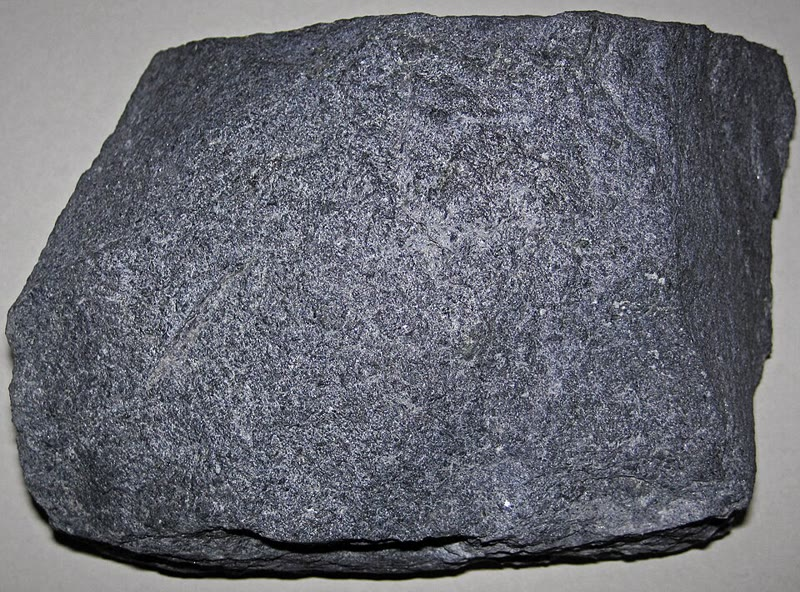
\includegraphics[height=4.4cm]{images/book2/g11-stjohn-blueschist.jpg}\hspace{0.03\linewidth}%
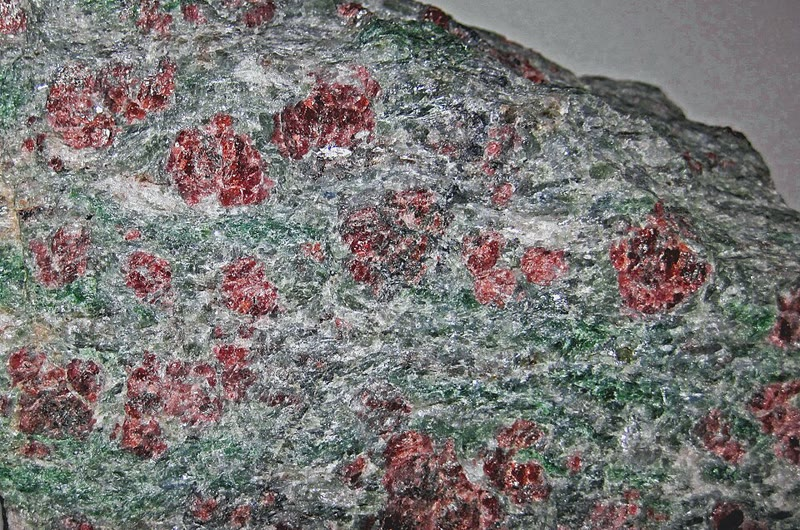
\includegraphics[height=4.4cm]{images/book2/g11-stjohn-eclogite.jpg}

{\small Links: \omterm{def:g11:subduction-zones:eclogite}{blauwschist} van Santa Catalina Island, Californië, ooit \omterm{def:g11:ocean-ridges:oceanic-lithosphere}{oceanische
korst} die in een \omterm{def:g11:subduction-zones:subduction}{subductiezone} is begraven. Rechts: \omterm{def:g11:subduction-zones:eclogite}{eclogiet} uit Noorwegen, met rode
granaten in groene pyroxeen. Foto's James St.~John (CC~BY~2.0).}
\end{omfigure}
% ledger: photo:g11-blueschist, photo:g11-eclogite

\omterm{def:g11:subduction-zones:eclogite}{Eclogiet} is dichter dan basalt; het is zelfs dichter dan de \omterm{def:g11:ocean-ridges:peridotite}{peridotiet} van de
mantel, met ongeveer \qty{6}{\percent}. Zodra zijn korst in \omterm{def:g11:subduction-zones:eclogite}{eclogiet} is veranderd,
draagt de \omterm{def:g11:subduction-zones:slab}{slab} geen lichte laag meer bovenop: de hele \omterm{def:g11:subduction-zones:slab}{slab} is dichter
dan de mantel eromheen, en trekt harder. Zulke gesteenten, die door latere bewegingen
weer aan het oppervlak zijn gebracht, behoren tot de weinige directe getuigen van
wat er tientallen kilometers diep in een \omterm{def:g11:subduction-zones:subduction}{subductiezone} gebeurt.
% ledger: hacker03:eclogite, photo:g11-eclogite

\begin{omfigure}
\begin{tikzpicture}[font=\footnotesize, scale=0.85]
  % subduction zone, a drawing, not to scale: slab top flat to x = -1, then bends to a 42-degree dip
  % coordinates computed once by a small script (scratch, not kept): slab top flat to x=-1, arc R=3 to a 42-degree dip
  \fill[omProp!10] (-7,-1.4) rectangle (7,-6.0);
  \fill[omSea!45] (-7,0) -- (-1,0) -- (1.6,0.8) -- (-7,0.8) -- cycle;
  \fill[lith peridotite] (-7.000,0.000) -- (-6.644,0.000) -- (-6.289,0.000) -- (-5.933,0.000) -- (-5.578,0.000) -- (-5.222,0.000) -- (-4.867,0.000) -- (-4.511,0.000) -- (-4.156,0.000) -- (-3.800,0.000) -- (-3.445,0.000) -- (-3.089,0.000) -- (-2.734,0.000) -- (-2.378,0.000) -- (-2.023,0.000) -- (-1.667,0.000) -- (-1.312,0.000) -- (-0.956,-0.000) -- (-0.602,-0.027) -- (-0.253,-0.094) -- (0.085,-0.203) -- (0.408,-0.351) -- (0.712,-0.536) -- (0.991,-0.756) -- (1.255,-0.994) -- (1.519,-1.232) -- (1.784,-1.470) -- (2.048,-1.707) -- (2.312,-1.945) -- (2.576,-2.183) -- (2.840,-2.421) -- (3.105,-2.659) -- (3.369,-2.897) -- (3.633,-3.135) -- (3.897,-3.373) -- (4.161,-3.611) -- (4.426,-3.848) -- (4.690,-4.086) -- (4.954,-4.324) -- (5.218,-4.562) -- (5.483,-4.800) -- (4.546,-5.840) -- (4.282,-5.603) -- (4.017,-5.365) -- (3.753,-5.127) -- (3.489,-4.889) -- (3.225,-4.651) -- (2.961,-4.413) -- (2.696,-4.175) -- (2.432,-3.937) -- (2.168,-3.699) -- (1.904,-3.461) -- (1.639,-3.224) -- (1.375,-2.986) -- (1.111,-2.748) -- (0.847,-2.510) -- (0.583,-2.272) -- (0.318,-2.034) -- (0.062,-1.803) -- (-0.087,-1.686) -- (-0.249,-1.587) -- (-0.421,-1.508) -- (-0.602,-1.450) -- (-0.788,-1.414) -- (-0.977,-1.400) -- (-1.312,-1.400) -- (-1.667,-1.400) -- (-2.023,-1.400) -- (-2.378,-1.400) -- (-2.734,-1.400) -- (-3.089,-1.400) -- (-3.445,-1.400) -- (-3.800,-1.400) -- (-4.156,-1.400) -- (-4.511,-1.400) -- (-4.867,-1.400) -- (-5.222,-1.400) -- (-5.578,-1.400) -- (-5.933,-1.400) -- (-6.289,-1.400) -- (-6.644,-1.400) -- (-7.000,-1.400) -- cycle;
  \fill[lith basalt] (-7.000,0.000) -- (-6.644,0.000) -- (-6.289,0.000) -- (-5.933,0.000) -- (-5.578,0.000) -- (-5.222,0.000) -- (-4.867,0.000) -- (-4.511,0.000) -- (-4.156,0.000) -- (-3.800,0.000) -- (-3.445,0.000) -- (-3.089,0.000) -- (-2.734,0.000) -- (-2.378,0.000) -- (-2.023,0.000) -- (-1.667,0.000) -- (-1.312,0.000) -- (-0.956,-0.000) -- (-0.602,-0.027) -- (-0.253,-0.094) -- (0.085,-0.203) -- (0.408,-0.351) -- (0.712,-0.536) -- (0.991,-0.756) -- (1.255,-0.994) -- (1.519,-1.232) -- (1.784,-1.470) -- (2.048,-1.707) -- (2.312,-1.945) -- (2.576,-2.183) -- (2.840,-2.421) -- (3.105,-2.659) -- (3.369,-2.897) -- (3.633,-3.135) -- (3.897,-3.373) -- (4.161,-3.611) -- (4.426,-3.848) -- (4.690,-4.086) -- (4.954,-4.324) -- (5.218,-4.562) -- (5.483,-4.800) -- (5.282,-5.023) -- (5.018,-4.785) -- (4.753,-4.547) -- (4.489,-4.309) -- (4.225,-4.071) -- (3.961,-3.833) -- (3.697,-3.596) -- (3.432,-3.358) -- (3.168,-3.120) -- (2.904,-2.882) -- (2.640,-2.644) -- (2.376,-2.406) -- (2.111,-2.168) -- (1.847,-1.930) -- (1.583,-1.692) -- (1.319,-1.455) -- (1.054,-1.217) -- (0.792,-0.980) -- (0.541,-0.783) -- (0.268,-0.616) -- (-0.023,-0.483) -- (-0.328,-0.385) -- (-0.642,-0.324) -- (-0.960,-0.300) -- (-1.312,-0.300) -- (-1.667,-0.300) -- (-2.023,-0.300) -- (-2.378,-0.300) -- (-2.734,-0.300) -- (-3.089,-0.300) -- (-3.445,-0.300) -- (-3.800,-0.300) -- (-4.156,-0.300) -- (-4.511,-0.300) -- (-4.867,-0.300) -- (-5.222,-0.300) -- (-5.578,-0.300) -- (-5.933,-0.300) -- (-6.289,-0.300) -- (-6.644,-0.300) -- (-7.000,-0.300) -- cycle;
  \fill[blue!30] (2.484,-2.100) -- (2.604,-2.208) -- (2.725,-2.317) -- (2.845,-2.425) -- (2.965,-2.533) -- (3.085,-2.642) -- (3.206,-2.750) -- (3.326,-2.858) -- (3.446,-2.967) -- (3.567,-3.075) -- (3.687,-3.183) -- (3.807,-3.292) -- (3.928,-3.400) -- (3.727,-3.623) -- (3.607,-3.515) -- (3.486,-3.406) -- (3.366,-3.298) -- (3.246,-3.190) -- (3.125,-3.081) -- (3.005,-2.973) -- (2.885,-2.865) -- (2.764,-2.756) -- (2.644,-2.648) -- (2.524,-2.540) -- (2.403,-2.431) -- (2.283,-2.323) -- cycle;
  \fill[lith eclogite] (3.928,-3.400) -- (4.057,-3.517) -- (4.187,-3.633) -- (4.316,-3.750) -- (4.446,-3.867) -- (4.576,-3.983) -- (4.705,-4.100) -- (4.835,-4.217) -- (4.964,-4.333) -- (5.094,-4.450) -- (5.223,-4.567) -- (5.353,-4.683) -- (5.483,-4.800) -- (5.282,-5.023) -- (5.152,-4.906) -- (5.023,-4.790) -- (4.893,-4.673) -- (4.764,-4.556) -- (4.634,-4.440) -- (4.504,-4.323) -- (4.375,-4.206) -- (4.245,-4.090) -- (4.116,-3.973) -- (3.986,-3.856) -- (3.857,-3.740) -- (3.727,-3.623) -- cycle;
  \draw[black!60] (-7.000,0.000) -- (-6.644,0.000) -- (-6.289,0.000) -- (-5.933,0.000) -- (-5.578,0.000) -- (-5.222,0.000) -- (-4.867,0.000) -- (-4.511,0.000) -- (-4.156,0.000) -- (-3.800,0.000) -- (-3.445,0.000) -- (-3.089,0.000) -- (-2.734,0.000) -- (-2.378,0.000) -- (-2.023,0.000) -- (-1.667,0.000) -- (-1.312,0.000) -- (-0.956,-0.000) -- (-0.602,-0.027) -- (-0.253,-0.094) -- (0.085,-0.203) -- (0.408,-0.351) -- (0.712,-0.536) -- (0.991,-0.756) -- (1.255,-0.994) -- (1.519,-1.232) -- (1.784,-1.470) -- (2.048,-1.707) -- (2.312,-1.945) -- (2.576,-2.183) -- (2.840,-2.421) -- (3.105,-2.659) -- (3.369,-2.897) -- (3.633,-3.135) -- (3.897,-3.373) -- (4.161,-3.611) -- (4.426,-3.848) -- (4.690,-4.086) -- (4.954,-4.324) -- (5.218,-4.562) -- (5.483,-4.800);
  \draw[black!60] (-7.000,-1.400) -- (-6.644,-1.400) -- (-6.289,-1.400) -- (-5.933,-1.400) -- (-5.578,-1.400) -- (-5.222,-1.400) -- (-4.867,-1.400) -- (-4.511,-1.400) -- (-4.156,-1.400) -- (-3.800,-1.400) -- (-3.445,-1.400) -- (-3.089,-1.400) -- (-2.734,-1.400) -- (-2.378,-1.400) -- (-2.023,-1.400) -- (-1.667,-1.400) -- (-1.312,-1.400) -- (-0.977,-1.400) -- (-0.788,-1.414) -- (-0.602,-1.450) -- (-0.421,-1.508) -- (-0.249,-1.587) -- (-0.087,-1.686) -- (0.062,-1.803) -- (0.318,-2.034) -- (0.583,-2.272) -- (0.847,-2.510) -- (1.111,-2.748) -- (1.375,-2.986) -- (1.639,-3.224) -- (1.904,-3.461) -- (2.168,-3.699) -- (2.432,-3.937) -- (2.696,-4.175) -- (2.961,-4.413) -- (3.225,-4.651) -- (3.489,-4.889) -- (3.753,-5.127) -- (4.017,-5.365) -- (4.282,-5.603) -- (4.546,-5.840);
  \draw[black!60] (5.483,-4.800) -- (4.546,-5.840);
  \fill[omLithGranite!55] (-1.000,0.000) -- (1.600,0.800) -- (7.000,0.800) -- (7.000,-1.600) -- (1.929,-1.600) -- (1.801,-1.485) -- (1.673,-1.370) -- (1.545,-1.255) -- (1.417,-1.140) -- (1.290,-1.025) -- (1.162,-0.910) -- (1.034,-0.795) -- (0.904,-0.682) -- (0.768,-0.577) -- (0.627,-0.479) -- (0.480,-0.390) -- (0.328,-0.310) -- (0.172,-0.238) -- (0.011,-0.176) -- (-0.152,-0.122) -- (-0.318,-0.078) -- (-0.487,-0.044) -- (-0.657,-0.020) -- (-0.828,-0.005) -- (-1.000,0.000) -- cycle;
  \fill[omLithAlluv] (-1.000,0.000) -- (0.550,0.470) -- (0.926,-0.700) -- (0.761,-0.571) -- (0.588,-0.455) -- (0.407,-0.350) -- (0.219,-0.259) -- (0.025,-0.180) -- (-0.174,-0.116) -- (-0.377,-0.065) -- (-0.583,-0.029) -- (-0.791,-0.007) -- (-1.000,0.000) -- cycle;
  \draw[black!60] (-1.000,0.000) -- (1.600,0.800) -- (7.000,0.800) -- (7.000,-1.600) -- (1.929,-1.600) -- (1.801,-1.485) -- (1.673,-1.370) -- (1.545,-1.255) -- (1.417,-1.140) -- (1.290,-1.025) -- (1.162,-0.910) -- (1.034,-0.795) -- (0.904,-0.682) -- (0.768,-0.577) -- (0.627,-0.479) -- (0.480,-0.390) -- (0.328,-0.310) -- (0.172,-0.238) -- (0.011,-0.176) -- (-0.152,-0.122) -- (-0.318,-0.078) -- (-0.487,-0.044) -- (-0.657,-0.020) -- (-0.828,-0.005) -- (-1.000,0.000);
  \draw[omThm!75, densely dashed, line width=0.7pt] (-7.000,-1.150) -- (-6.648,-1.150) -- (-6.296,-1.150) -- (-5.945,-1.150) -- (-5.593,-1.150) -- (-5.241,-1.150) -- (-4.889,-1.150) -- (-4.538,-1.150) -- (-4.186,-1.150) -- (-3.834,-1.150) -- (-3.482,-1.150) -- (-3.130,-1.150) -- (-2.779,-1.150) -- (-2.427,-1.150) -- (-2.075,-1.150) -- (-1.723,-1.150) -- (-1.372,-1.150) -- (-1.020,-1.150) -- (-0.796,-1.161) -- (-0.582,-1.198) -- (-0.374,-1.259) -- (-0.175,-1.344) -- (0.013,-1.452) -- (0.187,-1.581) -- (0.419,-1.788) -- (0.680,-2.023) -- (0.942,-2.259) -- (1.203,-2.494) -- (1.465,-2.730) -- (1.726,-2.965) -- (1.987,-3.200) -- (2.249,-3.436) -- (2.510,-3.671) -- (2.772,-3.907) -- (3.033,-4.142) -- (3.294,-4.377) -- (3.556,-4.613) -- (3.817,-4.848) -- (4.079,-5.083) -- (4.340,-5.319) -- (4.602,-5.554) -- (5.103,-4.997) -- (5.045,-4.944) -- (4.987,-4.892) -- (4.929,-4.839) -- (4.870,-4.787) -- (4.812,-4.734) -- (4.754,-4.682) -- (4.695,-4.629) -- (4.637,-4.577) -- (4.579,-4.524) -- (4.520,-4.472) -- (4.462,-4.419) -- (4.404,-4.367) -- (4.346,-4.315) -- (4.287,-4.262) -- (4.229,-4.210) -- (4.171,-4.157) -- (4.112,-4.105) -- (4.054,-4.052) -- (3.996,-4.000) -- (3.937,-3.947) -- (3.879,-3.895) -- (3.821,-3.842) -- (3.763,-3.790) -- (3.704,-3.737) -- (3.646,-3.685) -- (3.588,-3.632) -- (3.529,-3.580) -- (3.471,-3.527) -- (3.413,-3.475) -- (3.355,-3.422) -- (3.296,-3.370) -- (3.238,-3.317) -- (3.180,-3.265) -- (3.121,-3.212) -- (3.063,-3.160) -- (3.005,-3.107) -- (2.946,-3.055) -- (2.888,-3.002) -- (2.830,-2.950) -- (2.772,-2.897) -- (7.000,-2.897);
  \foreach \p in {(-0.72,-0.22),(-0.46,-0.36),(-0.18,-0.37),(0.05,-0.55),(0.29,-0.67),(0.63,-0.66),(0.87,-0.82),(0.91,-1.23),(1.27,-1.29),(1.50,-1.49),(1.55,-1.89),(1.90,-1.96),(2.04,-2.25),(2.35,-2.36),(2.54,-2.61),(2.88,-2.69),(2.99,-3.02),(3.16,-3.28),(3.47,-3.40),(3.65,-3.66),(3.89,-3.84),(4.26,-3.89),(4.32,-4.27),(4.59,-4.43),(4.88,-4.56),(5.17,-4.70)} \fill[black] \p circle (1.3pt);
  % volcanic arc above the slab, back-arc stretched
  \fill[black!70] (3.35,0.8) -- (3.7,1.4) -- (4.05,0.8) -- cycle;
  \draw[black!45, dashed] (5.2,0.8) -- (5.2,-1.6); \draw[black!45, dashed] (6.6,0.8) -- (6.6,-1.6);
  \draw[{Stealth[length=4pt]}-{Stealth[length=4pt]}, black!70] (5.35,-0.7) -- (6.45,-0.7);
  % motion arrows
  \draw[-{Stealth[length=5pt]}, line width=1pt] (-5.6,0.4) -- (-3.6,0.4);
  \draw[-{Stealth[length=5pt]}, line width=1pt] (1.77,-4.01) -- (2.88,-5.01);
  % labels
  \draw[black!60] (-1.0,0.02) -- (-1.8,1.05);
  \node[anchor=south] at (-1.8,1.05) {trog};
  \draw[black!60] (0.1,0.12) -- (0.5,1.05);
  \node[anchor=south, align=center] at (0.6,1.05) {afgeschraapte\\sedimenten};
  \node[anchor=south] at (2.35,0.85) {voorboog};
  \node[anchor=south] at (3.7,1.4) {vulkanische boog};
  \node[anchor=south] at (5.9,0.85) {achterboog};
  \node[anchor=south] at (-5.4,0.82) {oceaanbodem op weg naar de trog};
  \draw[black!60] (-7.0,-0.15) -- (-7.25,-0.15);
  \node[anchor=east] at (-7.25,-0.15) {oceanische korst};
  \draw[black!60] (-7.0,-0.85) -- (-7.25,-0.85);
  \node[anchor=east, align=right] at (-7.25,-0.85) {manteldeel van\\de lithosfeer};
  \node at (-3.5,-3.6) {asthenosfeer};
  \node[rotate=-42] at (3.98,-4.46) {slab};
  \draw[black!60] (3.35,-2.65) -- (4.3,-2.35);
  \node[anchor=west] at (4.3,-2.35) {blauwschist};
  \draw[black!60] (5.1,-4.3) -- (5.75,-4.6);
  \node[anchor=west] at (5.75,-4.6) {eclogiet};
  \node[anchor=north east, text=omThm!80!black, align=right] at (7,-2.95) {lijn van gelijke\\temperatuur};
  \fill[black] (-6.8,-5.55) circle (1.3pt);
  \node[anchor=west] at (-6.65,-5.55) {aardbevingen};
\end{tikzpicture}

{\small Een \omterm{def:g11:subduction-zones:subduction}{subductiezone} (een tekening, niet op schaal). Oude \omterm{def:g11:ocean-ridges:oceanic-lithosphere}{oceanische lithosfeer}
buigt bij de trog naar beneden en zakt onder de bovenliggende plaat weg. Sedimenten
die van zijn oppervlak zijn afgeschraapt, stapelen zich op tegen de rand van de
bovenliggende plaat; de aardbevingen volgen de wegzakkende \omterm{def:g11:subduction-zones:slab}{slab}; zijn korst verandert in
\omterm{def:g11:subduction-zones:eclogite}{blauwschist}, en dan in \omterm{def:g11:subduction-zones:eclogite}{eclogiet}. De \omterm{def:g11:subduction-zones:slab}{slab} blijft kouder dan de mantel eromheen: de
lijnen van gelijke temperatuur worden erlangs naar beneden meegetrokken. Een rij vulkanen, de
vulkanische boog, staat boven de \omterm{def:g11:subduction-zones:slab}{slab}.}
\end{omfigure}
% volcanic arc above the slab: told only, defined and sourced in g12.04

\section{De anatomie van een subductiezone}

Van de oceaan naar het continent, of naar de volgende oceaan, heeft een \omterm{def:g11:subduction-zones:subduction}{subductiezone}
altijd dezelfde delen.

\begin{itemize}
  \item De \emph{trog}, waar de wegzakkende plaat naar beneden buigt: de diepste
        plaatsen van de oceanen.
  \item De \emph{voorboog}, tussen de trog en de rij vulkanen. Zijn
        rand is een stapel sedimenten die van de wegzakkende plaat zijn afgeschraapt; eronder
        schuiven de twee platen langs elkaar langs de plaatgrens, een
        flauw hellende breuk waarop zware aardbevingen plaatsvinden, zoals
        die van 2011 voor de kust van Japan (voorbeeld hieronder).
  \item De \emph{vulkanische boog}, een rij vulkanen evenwijdig aan de trog,
        op eilanden (Tonga, de Marianen, Japan) of op een continent (de Andes);
        waarom die ontstaat, is het onderwerp van \cref{ch:g12:subduction-magmatism}.
  \item Achter sommige bogen een \emph{achterboog}, waar de bovenliggende plaat wordt
        uitgerekt; achter Tonga wordt ze uit elkaar getrokken.
\end{itemize}
% ledger: bevis95:tonga (back-arc extension at Tonga); usgs:tohoku (largest earthquakes on the
% plate boundary: example below)

Achter Tonga voert de uitrekking van de achterboog de boog zelf naar de
Pacifische plaat toe, zoals satellietplaatsbepaling heeft laten zien. De snelheid waarmee de twee kanten van de Tongatrog convergeren,
is daarom groter dan de eigen snelheid van elk van beide platen: volgens het model PB2002
ongeveer \qty{17}{cm} per jaar bij \ang{20}~ZB.
% values: tonga_rate 168.0 (mean of the PB2002 TO/PA steps within 100 km of the profile);
% PB2002 steps along Tonga: 104 to 237 mm/yr; ledger data:pb2002, bevis95:tonga

\begin{example}[De aardbeving van Tōhoku, 2011]\label{ex:g11:subduction-zones:tohoku}
Op 11~maart 2011 trof een aardbeving met magnitude 9.1 de zee voor de noordoostkust
van Honshu, Japan. Ze vond ongeveer \qty{25}{km} diep plaats, op de plaatgrens
zelf, waar de Pacifische plaat, die met ongeveer \qty{83}{mm} per
jaar naar het westen beweegt ten opzichte van de plaat die het noorden van Japan draagt, er bij
de Japantrog onder wegzakt. De twee kanten van de breuk schoven tot wel 50 à
\qty{60}{m} langs elkaar, over een gebied van ongeveer \qty{400}{km} lang en
\qty{150}{km} breed. De zeebodem erboven bewoog mee, en veroorzaakte een tsunami
die tot \qty{38}{m} hoog tegen de kust opliep; minstens \num{15703} mensen kwamen
om en \num{4647} werden vermist. Dezelfde kust was al getroffen door
tsunami's uit deze \omterm{def:g11:subduction-zones:subduction}{subductiezone} in 1611, 1896 en 1933, en misschien door een
die even groot was als die van 2011 in het jaar 869.
\end{example}
% ledger: usgs:tohoku

\begin{omfigure}
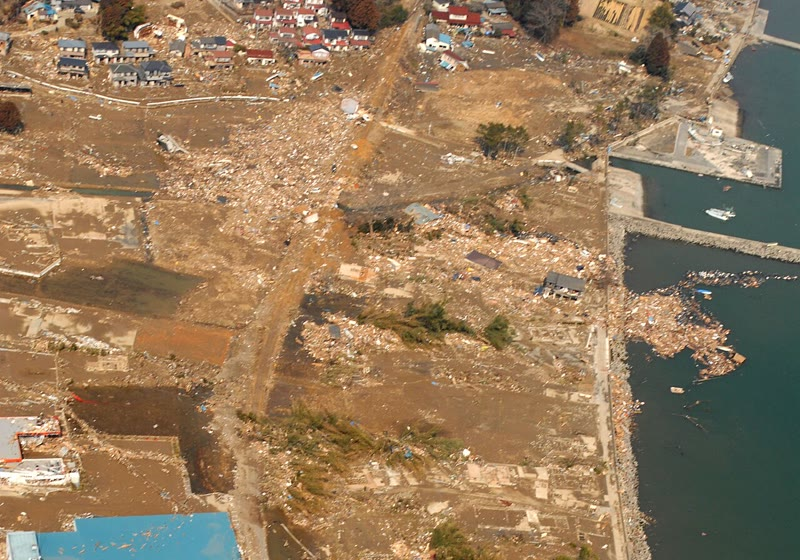
\includegraphics[width=0.78\linewidth]{images/book2/g11-usn-tsunami-kesennuma.jpg}

{\small De vissershaven van Kesennuma, aan de noordoostkust van Japan, twee
dagen na de tsunami van 11~maart 2011. Foto Dylan McCord, U.S. Navy
(publiek domein).}
\end{omfigure}
% ledger: photo:g11-tsunami

\section{Oefeningen}

\begin{exercise}[$\star$]\label{exo:g11:subduction-zones:1}
Definieer \omterm{def:g11:subduction-zones:subduction}{subductie} en een \omterm{def:g11:subduction-zones:subduction}{subductiezone}. Welk soort \omterm{def:g11:lithosphere-asthenosphere:lithosphere}{lithosfeer} zakt bij een
\omterm{def:g11:subduction-zones:subduction}{subductiezone} weg, en waarom dat soort?
\end{exercise}

\begin{exercise}[$\star$]\label{exo:g11:subduction-zones:2}
Gebruik de wereldkaart van aardbevingen naar diepte: (1) noem drie gebieden met
aardbevingen dieper dan \qty{300}{km}; (2) aan welke kant van een trog liggen de
diepe aardbevingen? (3) Hoe diep zijn de aardbevingen langs de Midden-Atlantische
Rug?
\end{exercise}

\begin{exercise}[$\star$]\label{exo:g11:subduction-zones:3}
De catalogus bevat \num{7031} aardbevingen met magnitude 6 of meer, waarvan
\qty{21}{\percent} dieper dan \qty{70}{km} en \qty{6.9}{\percent} dieper
dan \qty{300}{km}. Hoeveel aardbevingen zijn dat in elk geval?
\end{exercise}

\begin{exercise}[$\star$]\label{exo:g11:subduction-zones:4}
Definieer \omterm{def:g11:subduction-zones:eclogite}{blauwschist} en \omterm{def:g11:subduction-zones:eclogite}{eclogiet}. Wat hebben beide gemeen met het basalt
van de \omterm{def:g11:ocean-ridges:oceanic-lithosphere}{oceanische korst}? Wat verschilt er?
\end{exercise}

\begin{exercise}[$\star$]\label{exo:g11:subduction-zones:5}
Noem de delen van een \omterm{def:g11:subduction-zones:subduction}{subductiezone} op volgorde, van de oceaanbodem die
naar de trog beweegt tot de achterboog, en zeg in één regel wat er in
elk deel gebeurt.
\end{exercise}

\begin{exercise}[$\star\star$]\label{exo:g11:subduction-zones:6}
Op de doorsnede door de Andes ligt de lijn die de aardbevingen volgt
\qty{135}{km} diep op \qty{300}{km} van de trog en \qty{508}{km} diep op
\qty{800}{km}. Bereken de helling van de \omterm{def:g11:subduction-zones:slab}{slab}.
\end{exercise}

\begin{exercise}[$\star\star$]\label{exo:g11:subduction-zones:7}
Een rechte \omterm{def:g11:subduction-zones:slab}{slab} begint bij een trog en helt onder \ang{45}. (1) Hoe diep ligt hij
op \qty{300}{km} van de trog? (2) Op welke afstand van de trog bereikt hij
\qty{670}{km}? (3) Welke lengte \omterm{def:g11:subduction-zones:slab}{slab} ligt er tussen de trog en
\qty{670}{km}?
\end{exercise}

\begin{exercise}[$\star\star$]\label{exo:g11:subduction-zones:8}
De gemiddelde snelheden van de platen zijn, in millimeter per jaar: Cocos 74.6, Nazca
70.0, Pacifisch 65.5, Australië 63.1, Filipijnse Zee 52.6 (met \omterm{def:g11:subduction-zones:slab}{slab}); Arabië
47.6, Somalië 31.0, Nubië 29.2, Eurazië 22.8, Noord-Amerika 19.8, Antarctica
15.2, Caribisch 14.9, Zuid-Amerika 10.6 (zonder). (1) Bereken het gemiddelde van
elke groep en hun verhouding. (2) Wat suggereert dit over de kracht die
de platen aandrijft?
\end{exercise}

\begin{exercise}[$\star\star$]\label{exo:g11:subduction-zones:9}
In 2011 schoof de breuk voor de kust van Japan tot wel 50 à \qty{60}{m}. De
Pacifische plaat nadert met \qty{83}{mm} per jaar. (1) Hoeveel jaar plaatbeweging
vormt een verschuiving van \qty{50}{m}, en dan van \qty{60}{m}? (2) Vergelijk met
de tijd sinds 869, een mogelijke eerdere aardbeving van dezelfde grootte.
\end{exercise}

\begin{exercise}[$\star\star$]\label{exo:g11:subduction-zones:10}
De oceaanbodem die de Japantrog bereikt, is ongeveer 133 miljoen jaar oud,
die bij Tonga ongeveer 99 en die bij de Andes ongeveer 49. (1) Bereken met
de wetten van \cref{ch:g11:ocean-ridges} ($2500 + 350\sqrt{t}$ voor
$t \le 70$, $6400 - 3200\,e^{-t/62.8}$ daarboven) de diepte van elk. (2)
Welke is de koudste en dichtste \omterm{def:g11:lithosphere-asthenosphere:lithosphere}{lithosfeer}?
\end{exercise}

\begin{exercise}[$\star\star$]\label{exo:g11:subduction-zones:11}
Het basalt van de \omterm{def:g11:ocean-ridges:oceanic-lithosphere}{oceanische korst} heeft een dichtheid van ongeveer \qty{2900}{kg/m^3},
de mantel rond de \omterm{def:g11:subduction-zones:slab}{slab} \qty{3380}{kg/m^3}, en \omterm{def:g11:subduction-zones:eclogite}{eclogiet} is
\qty{6}{\percent} dichter dan de mantel. (1) Bereken de dichtheid van \omterm{def:g11:subduction-zones:eclogite}{eclogiet}.
(2) Met welk percentage stijgt de dichtheid van de korst wanneer die in
\omterm{def:g11:subduction-zones:eclogite}{eclogiet} verandert? (3) Is de korst, ervoor en erna, lichter of dichter dan de
mantel, en met hoeveel?
\end{exercise}

\begin{exercise}[$\star\star\star$]\label{exo:g11:subduction-zones:12}
Warmte verspreidt zich door geleiding over een afstand van ongeveer $\sqrt{\kappa t}$ in een
tijd $t$, met $\kappa = \qty{1e-6}{m^2/s}$ voor gesteente. (1) Bereken deze afstand
voor 6 miljoen jaar ($1~\text{jaar} \approx \qty{3.16e7}{s}$). (2) Vergelijk ze
met de dikte van een \omterm{def:g11:subduction-zones:slab}{slab}, ongeveer \qty{100}{km}. (3) Leg uit waarom er
aardbevingen kunnen plaatsvinden in een \omterm{def:g11:subduction-zones:slab}{slab} op \qty{600}{km} terwijl de mantel eromheen
vloeit.
\end{exercise}
% ledger: england:kelvin (kappa 1e-6 m2/s)

\begin{exercise}[$\star\star\star$]\label{exo:g11:subduction-zones:13}
Onder de Andes op \ang{21}~ZB bereikt de lijn van de doorsnede
\qty{670}{km} op \qty{1017}{km} van de trog, en de platen convergeren met
\qty{64}{mm} per jaar. (1) Schat de lengte van de \omterm{def:g11:subduction-zones:slab}{slab} van de trog tot
\qty{670}{km}. (2) Hoe lang doet een stuk oceaanbodem erover om
\qty{670}{km} te bereiken? (3) Vergelijk met Tonga, waar dezelfde reis ongeveer 6
miljoen jaar duurt.
\end{exercise}

\begin{exercise}[$\star\star\star$]\label{exo:g11:subduction-zones:14}
Neem een \omterm{def:g11:subduction-zones:slab}{slab} van \qty{100}{km} dik, gemiddeld \qty{36}{kg/m^3} dichter dan de
mantel eromheen, en \qty{1000}{km} lang, onder een trog.
(1) Bereken het massaoverschot van de \omterm{def:g11:subduction-zones:slab}{slab} per meter trog. (2) Bereken
zijn gewicht, met $g = \qty{9.8}{m/s^2}$. (3) Waarom kan deze kracht de hele
plaat meetrekken?
\end{exercise}

\begin{exercise}[$\star\star\star$]\label{exo:g11:subduction-zones:15}
Langs de Tongatrog geeft het model PB2002 een convergentie van
\qty{104}{mm} per jaar op \ang{23.6}~ZB en \qty{237}{mm} per jaar op
\ang{16.5}~ZB. (1) Hoe ver liggen de twee punten uit elkaar, langs een meridiaan
($\ang{1} \approx \qty{111}{km}$)? (2) Hoeveel neemt de snelheid toe per
honderd kilometer? (3) De Pacifische plaat beweegt op beide punten met ongeveer
dezelfde snelheid. Wat moet de andere kant van de trog, de Tongaboog, dan doen?
\end{exercise}

\section{Probleem: de slab van Tonga}

\begin{problem}[{Weekendprobleem --- van de trog tot \qty{670}{km}}]
\label{pb:g11:subduction-zones:1}
% values: tonga fit -23.568 + 0.91068 x; tonga_rate 168.0 mm/yr; tonga_age 98.8;
% x670 761.6; path 1014; time 6.04 Myr; tonga_maxdepth 670.8 (slab_sections.py);
% MKEA 69 mm/yr (plate_velocities.py); kappa england:kelvin; eclogite hacker03:eclogite
Onder de Tongatrog zakt de Pacifische plaat naar het westen weg. Gebruik de doorsnede
door Tonga van dit hoofdstuk, waarvan de lijn $z = -24 + 0.91\,x$ is (beide in
kilometer, $x$ gemeten van de trog naar de boog).

\medskip
\noindent\textbf{Deel I --- De aardbevingsdoorsnede.}
\begin{enumerate}
  \item Hoe diep ligt de diepste aardbeving van de doorsnede?
  \item Waarom zijn er geen diepe aardbevingen aan de oceaankant van de trog?
  \item Bereken de diepte van de lijn bij $x = 300$ en $x = 700$, en dan de
        helling van de \omterm{def:g11:subduction-zones:slab}{slab}.
  \item Op welke horizontale afstand van de trog ligt de \omterm{def:g11:subduction-zones:slab}{slab}
        \qty{100}{km} diep? En \qty{400}{km} diep?
  \item De lijn ligt bij $x = 0$ \qty{24}{km} boven de trog. Wat zegt
        dit je over de vorm van de \omterm{def:g11:subduction-zones:slab}{slab} dicht bij de trog?
\end{enumerate}

\medskip
\noindent\textbf{Deel II --- De convergentie.}
\begin{enumerate}[resume]
  \item De platen convergeren over de trog met ongeveer \qty{168}{mm} per jaar.
        Reken om naar centimeter per jaar en kilometer per miljoen jaar.
  \item De Pacifische plaat beweegt boven Hawaii met ongeveer \qty{69}{mm} per jaar.
        Hoeveel keer sneller is de convergentie bij Tonga?
  \item Leg met de som van relatieve snelheden uit hoe de convergentie
        groter kan zijn dan de snelheid van de Pacifische plaat.
  \item De bodem die de trog bereikt, is ongeveer 99 miljoen jaar oud. Hoe
        diep ligt hij (exponentiële wet van \cref{ch:g11:ocean-ridges})?
  \item Waarom kan zo'n \omterm{def:g11:lithosphere-asthenosphere:lithosphere}{lithosfeer} uit zichzelf wegzakken?
\end{enumerate}

\medskip
\noindent\textbf{Deel III --- Tot \qty{670}{km}.}
\begin{enumerate}[resume]
  \item Op welke horizontale afstand van de trog bereikt de lijn
        \qty{670}{km}?
  \item Schat de lengte van de \omterm{def:g11:subduction-zones:slab}{slab} van de trog tot dat punt,
        als je hem als recht beschouwt.
  \item Hoe lang doet een stuk oceaanbodem erover om deze lengte af te leggen bij
        \qty{168}{mm} per jaar?
  \item Hoe lang zou het duren bij de \qty{69}{mm} per jaar van de Pacifische
        plaat boven Hawaii?
  \item Onderweg verandert de korst van de \omterm{def:g11:subduction-zones:slab}{slab} in \omterm{def:g11:subduction-zones:eclogite}{eclogiet},
        \qty{6}{\percent} dichter dan de mantel van \qty{3380}{kg/m^3}. Wat
        is zijn dichtheid, en wat verandert dit voor de \omterm{def:g11:subduction-zones:slab}{slab}?
\end{enumerate}

\medskip
\noindent\textbf{Deel IV --- Een koude slab in een hete mantel.}
\begin{enumerate}[resume]
  \item Gedurende de tijd van vraag~13 verspreidt warmte zich door geleiding over ongeveer
        $\sqrt{\kappa t}$, met $\kappa = \qty{1e-6}{m^2/s}$. Bereken deze
        afstand.
  \item Vergelijk ze met de dikte van de \omterm{def:g11:subduction-zones:slab}{slab}, ongeveer \qty{100}{km}. Is
        de \omterm{def:g11:subduction-zones:slab}{slab} vanbinnen nog koud wanneer hij \qty{670}{km} bereikt?
  \item Waarom verklaart dit de aardbevingen op \qty{600}{km} en dieper
        onder Tonga?
  \item Welke verandering in de mantel lieten seismische golven zien bij
        \qty{670}{km} (\cref{ch:g11:seismic-structure})?
  \item Besluit: hoe lang doet Pacifische oceaanbodem erover om van de
        Tongatrog tot \qty{670}{km} te zakken?
\end{enumerate}
\end{problem}
